\documentclass[11pt,leqno,oneside]{amsart}
%\usepackage[margin=1in]{geometry}

\usepackage{../notes}
\usepackage{xfrac}
\usepackage{enumitem}
\usepackage{tikz-cd}
\usetikzlibrary{cd}
\usepackage{hyperref}
\usepackage{amsrefs} % AMS references % must be loaded AFTER hyperref if you use that
\usepackage{mathtools}
\mathtoolsset{showonlyrefs}

\usepackage{datetime}
% an environment specifically for my dates, although it doesn't actually depend on datetime:
\newenvironment{dateenv}{
  \vspace{1em}
}{
  \vspace{1em}
}
% my date command, for convenient date adding
\newcommand{\mydate}[4]{
  \newdate{#1}{#2}{#3}{#4}
  % #1 is a unique string, #2 is day, #3 month, #4 year
  \begin{dateenv}
    \hfill\displaydate{#1}
  \end{dateenv}
}

\numberwithin{thm}{section}

\everymath{\displaystyle}


\newcommand{\minus}{\smallsetminus}
\renewcommand{\setminus}{\smallsetminus}
\renewcommand{\amalg}{\sqcup}
\renewcommand{\null}{\varnothing}
\newcommand{\homotopic}{\simeq}
\renewcommand{\epsilon}{\varepsilon}
\renewcommand{\d}{\partial}
\newcommand{\fund}[1][1]{\pi_{#1}}
\newcommand{\transverse}{\pitchfork}
\newcommand{\x}{\times}
\newcommand{\Map}{\text{Map}}
\newcommand{\Mor}{\text{Mor}}
\newcommand{\id}{\text{id}}
\newcommand{\adj}{\sim} % for 'adjacent' in a graph
\newcommand{\Arg}{\text{Arg}}
\renewcommand{\bar}{\widebar}

%%%%%%%%%%%%%% BEGIN CONTENT: %%%%%%%%%%%%%%

\title[Algebraic Topology]{Algebraic Topology MATH 7800}
\author{Chris Lloyd, Matthew Lancellotti}
\date{}
\begin{document}
\maketitle \newpage

\mydate{d1}{18}{1}{2017}

\section{Introduction}

Topology is floppy. Given just a topological space one has an infinite
degree of freedom. This makes even simple questions hard to answer, in
particular given manifolds \(M\) and \(N\) with different dimensions
\(m\) and \(n\) respectively, one may ask if they are
homeomorphic. Intuitively one would think that should not be
possible. However there do exist space filling curves, i.e,
\[I \twoheadrightarrow I \times I\]
where as always \(I=[0,1]\).

We will develop the tools to prove manifolds of different dimensions can
certainly never be homeomorphic. Another surface result assures there exists no continuous
retraction \(D^2 \to \d D^2\), which then immediately yields the
Brouwer Fixed Pointed Theorem (every map \(D^2 \to D^2\) admits a
fixed point).

In this course there will be two basic branches under consideration:
homotopy theory and homology. Basically, homotopy concerns itself with
continuous deformations between maps. While homology studies subspaces
(known as ``cycles'') and gap filling.

\section{Reference}
%
\begin{defn}
  $D^n$ denotes the $n$-dimensional closed unit disk.
\end{defn}

\section{Homotopy}

We now define homotopies in the space of maps between manifolds \(M\)
and \(N\) denoted
\[\Map(M,N)=\{f \from M \to N \mid \text{$f$ is continuous}\}.\]

In this course, we follow the convention that maps are continuous
functions unless otherwise stated!

\begin{defn}
  A \emph{homotopy} from \(f \in \Map(M, N)\) to \(g \in \Map(M, N)\) is a path in $\Map(M, N)$ that starts at $f$ and ends at $g$.  Therefore, $h_0 = f$ and $h_1 = g$.

  Equivalently, a \emph{homotopy} from \(f \from M \to N\) to \(g \from M \to N\)
  is a map \(h\from M \x I \to N\) such that \(h_0=f\) and \(h_1=g\). We say \(f\) and
  \(g\) are \emph{homotopic} if a homotopy between them exists.

  Often we write \(h_t(m)\) for \(h(m,t)\).
\end{defn}

When working with homotopies one often thinks of having the start and
end map already fixed. For maps to be homotopic they must be in the
same path component.

\begin{prop}
  Homotopy is an equivalence relation.
\end{prop}

We denote the homotopy equivalence class of \(f\) by \([f]\).

\begin{defn}
  A homotopy $h\from I \x X \to Y$ is called \de{relative} to a subset $A$ of $X$ if for all $a \in A$ and all $t \in I$, $h(a, t) = f(a) = g(a)$.

  We also say that ``$f$ and $g$ are homotopic relative to $A$''.
\end{defn}

When there are no restrictions placed on a homotopy, it is sometimes called a \emph{free} homotopy.

\begin{defn}
  A \emph{path} in a topological space $X$ is a map
  \[f \from I \to X.\]
\end{defn}

By convention in this course, we always consider paths up to homotopy relative to $\{0, 1\}$.  That means that our homotopies fix the end points.  If they didn't, every path would collapse to a point up to homotopy!

Imagine two paths in \(\R^2 \setminus (0,0)\) which agree on end points,
however each path is on opposite sides of the origin. It is clear that
there exists no end point fixing homotopy between the two paths.

\begin{defn}
  If one has two paths \(f,g\) with \(f(1)=g(0)\) we may define a new
  path
  \[f * g :=
    \begin{cases}
      f(2t), & t \in [0,\frac{1}{2})\\
      g(2t - 1), & t \in [\frac{1}{2},1].
    \end{cases}
  \]

  This is called the \emph{concatenation} or \emph{path composition}
  of $f$ and $g$.

  This operation is well defined on homotopy classes, that is if
  \([f]=[f']\) and \([g]=[g']\) then \([f * g] = [f' * g']\). This
  operation may be generalized to \(*_{k}\) where \(k \in (0,1)\),
  simply replace \(\frac{1}{2}\) with \(k\). In this notation
  \(f * g = f *_{\frac{1}{2}} g\). Concatenation is associative.
\end{defn}

Given a topological space \(X\) with points \(P\), for any two points
\(x,y \in P\) we have a set of homotopy classes with end points \(x\)
and \(y\). These may be thought of as morphisms and the points as
objects in a category. We call this category the Fundamental Groupoid.

\mydate{d2}{20}{1}{2017}

\begin{defn}[\cite{ncatlab}]
  A \de{category} $\mathcal{C}$ consists of
  \begin{itemize}
    \item A class of objects $\Ob(\mathcal{C})$
    \item For every pair of objects $A, B \in \Ob(\mathcal{C})$, a set $\Hom(A, B)$ of \de{morhpisms}
    \item A composition operation.  That is, if $f \in \Hom(A,B)$ and $g \in \Hom(B,C)$, then there exists a morphism $h \in \Hom(A,C)$ s.t. $h = f.g$, where ``.'' denotes the composition operation.  The composition operation must be associative.
    \item For every object $A \in \Ob(\mathcal{C})$, an \de{identity morphism} $\id_A\from A \to A$ s.t. for all $f\from A \to B$ we have $\id_A.f = f$ and for all $g\from B \to A$ we have $g.\id_A = g$, for all $B$.
  \end{itemize}
\end{defn}

\begin{defn}
  In the category of \de{finite sets}, denoted $\text{FSet}$, the
  objects are the finite sets, each morphism from $A$ to $B$ is a
  function from $A$ to $B$.
\end{defn}
\begin{defn}
  For any field $K$, the category of \de{$K$-vector spaces} (vector spaces over $K$), denoted
  $\text{Vect}_K$, has objects that are $K$-vector spaces and
  morphisms that are $K$-linear maps.
\end{defn}
\begin{defn}
  A \de{groupoid} is a category where every morphism has an inverse.

  That is, for any objects $x$ and $x'$ and any morphism $a \from x \to x'$ between them, there exists $a^{-1} \from x' \to x$
  s.t. $aa^{-1} = \id_{x'}$ and $a^{-1}a = \id_{x}$.
\end{defn}
\begin{rmk}
  A groupoid can be viewed as a more general notion than a group!

  The elements of the groupoid are the morphisms.  The operation is composition.  Not every pair of morphisms can necessarily be composed!

  So a groupoid is just like a group, but not every pair of elements can be multiplied!  Also, there is not a \textbf{single} identity, but rather, there could be many left and right identities.  That is, each object has a little loop.
\end{rmk}
\begin{prop}
  Every morphism in a groupoid is an isomorphism (by definition).
\end{prop}
\begin{defn}
  A \de{group} is a groupoid with one object.
\end{defn}
\begin{prop}
  If $A$ is an object in a groupoid, then $\Hom(A, A)$ is a group.
\end{prop}

Note, we see that a groupoid is the same definition of a group, but we
use a *partial* binary operation instead of a binary operation.

\begin{defn}
  The \de{fundamental groupoid} of $X$, denoted $\Pi_1 X$, is the
  category where the objects are the points in $X$ and the morphisms
  are the paths (up to endpoint fixing homotopy) between those points.
\end{defn}
\begin{defn}
  The \de{fundamental group of $X$ at the basepoint $x_0$}, denoted
  $\fund(X, x_0)$, is the subgroupoid of the fundamental groupoid
  where there is exactly one object, $x_0$, and the morphisms are the
  morphisms of the fundamental groupoid that have source and target
  $x_0$.  Another wording is to say that $\fund(X, x_0)$ is the full
  subcategory of $\Pi_1 X$ spanned by $x_0$.

  The elements of the group are the morphisms.  The operation is
  composition.
\end{defn}
\begin{defn}
  The \de{inverse path} of a path $p$ is $p^{-1}(s) := p(1-s)$.  In Hatcher, this is denoted $\bar{p}$.
  (Note: This is *not* the same as the function inverse of $p$)
\end{defn}
\begin{prop}
  If $p$ is a path, then
  $[p^{-1}*p] = [id_{x}]$, which is the equivalence class of the
  function where $s \mapsto x$ for
  all $s \in [0,1]$.
\end{prop}

\begin{thm}[Hatcher 1.5]
  Let $X$ be a metric space and $x,x' \in X$.  If there exists
  $p\from x \to x'$ and $[q] \in \fund(X,x')$, then
  $p^{-1}qp \in \fund(X,x)$.  The ``conjugacy'' map that sends each $[q]$ to $[p^{-1}qp]$ is an isomorphism of fundamental groups.
\end{thm}
\begin{thm}
  If $X$ is path connected, then for any $x_a, x_b \in X$,
  $$\fund(X, x_a) \isom \fund(X, x_b).$$
\end{thm}
In the above situation, we can denote the fundamental
group with $\fund(X)$ or $\fund X$.
\begin{example}
  The isomorphism above is not canonical, because we could use path $p$ or $q$ to create the isomorphism, but $p$ and $q$ are not homotopic, as shown below.

  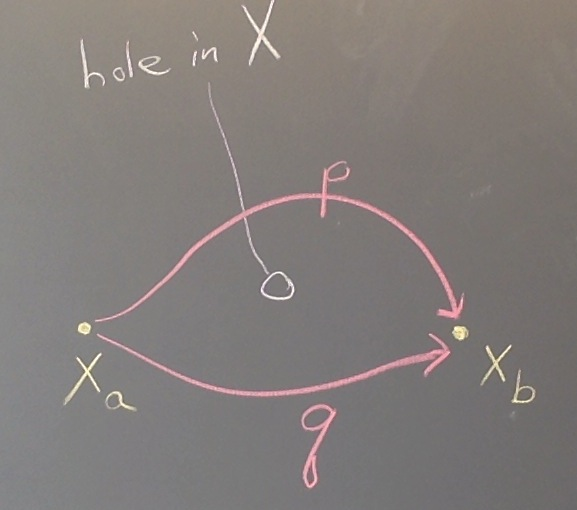
\includegraphics[scale=0.2]{images/isomorphism-not-canonical}

  Note that $\fund X$ is only well defined up to inner automorphism.  ((What does this mean?))
\end{example}
\begin{defn}
  Given spaces $X, Y$ and a map $f\from X \to Y$, then the
  \de{fundamental functor} induced by $f$,
  $$f_* = \Pi_1 f \from \Pi_1 X \to \Pi_1 Y$$ maps each object $x \in X$
  to $f(x) \in Y$ and each path $[p] \in \Pi_1 X$ to
  $f([p]) = [f(p)] \in \Pi_1 Y$.
\end{defn}
\begin{prop}
  The above is well defined because
  \begin{itemize}
  \item If $[p]=[q]$, then $[f(p)] = [f(q)]$.  Proof:  Consider the homotopy $h$ s.t. $h_0 = p$ and $h_1 = q$.  $f$ is continuous, so $h.f$ is a homotopy, and $(h.f)_0 = f(p)$ and $(h.f)_1 = f(q)$.
  \item If $p$ and $q$ represent equivalence classes, and if they can be concatenated, then $(f_*p)*(f_*q) = f_*(p*q)$.
  \end{itemize}
\end{prop}

\begin{prop}
  Given a fundamental group $\fund(X, x)$, then we can restrict $f_*$
  to the functor $$f_* \from \fund(X, x) \to \fund(Y, f(x)).$$ which is a group homomorphism.

  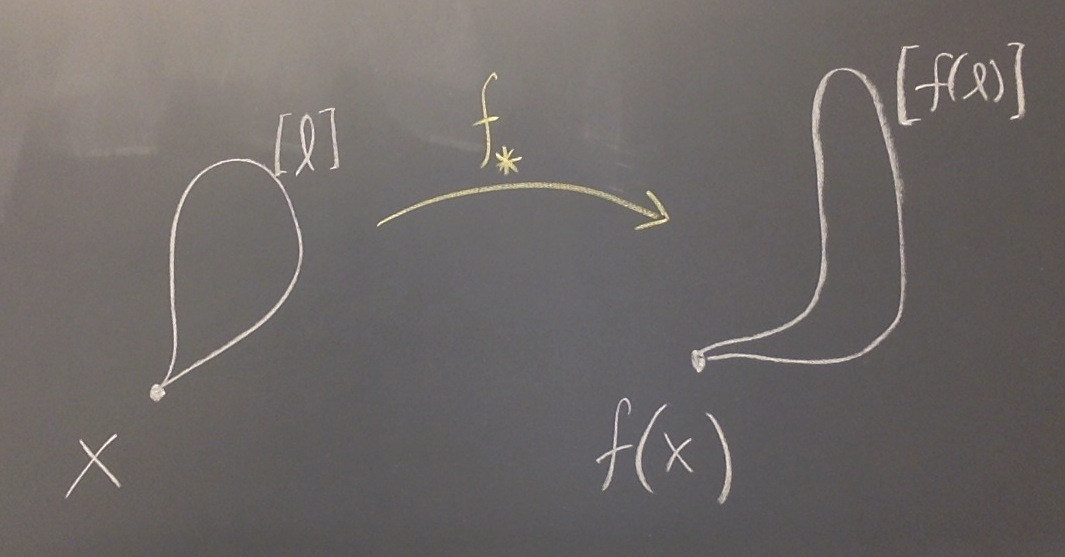
\includegraphics[scale=0.17]{images/fundamental-functor}
\end{prop}
\begin{prop}
  If $X,Y,Z$ are metric spaces and $f \from X \to Y$, $g \from Y \to Z$ are
  maps, then ${(f.g)}_* = f_*.g_*$.
\end{prop}

\begin{example}
  $\fund(\R^n, x) = \{[*]\} = \{e\}$

  In $\Pi_1 \R^n$, there exists a unique path between any two points,
  up to homotopy.

  Note that $\fund(B_n) = \{e\}$ and $\fund(I_n) = \{e\}$ too!
\end{example}
\begin{proof}
  Let $p,q \from I \to \R^n$ be any two paths that satisfy $p(0) = q(0)$ and $p(1) = q(1)$.

  Define $h$ by $h_t = tp + (1-t)q$.  It follows that, $h_0 = q$, $h_1 = p$, and $h$ is a homotopy.
\end{proof}

\begin{defn} % I'm pretty sure this is the DEFINITION of simply connected.  We're just saying "the fundamental group is trivial" instead of saying "every loop can be shrunk continuously to a point".  I suppose we could create a separate definition if you wish.  Also, Hatcher 1.6 doesn't exist.
  A space $X$ is \de{simply connected} or \de{1-connected} iff it is path connected and its
  fundamental group is trivial.
\end{defn}
\begin{example}
  $\R^2 \minus (0,0) \isom \C \minus \{0\}$ is NOT simply connected.
  $\fund(\C \minus \{0\}) = \Z$
\end{example}
\begin{example}
  Consider a loop $A$ that goes around a hole in $X$ once, and a loop $B$ that looks exactly the same as $A$, but it goes around the hole in $X$ twice.

  $A$ and $B$ can't be homotopic because $\Arg(A)$ and $\Arg(B)$ have
  different end points.
\end{example}

\begin{defn}
  A \emph{covering space} \((\tilde{X},p)\) of a space \(X\) is a space \(\tilde{X}\)
  and map \(p \from \tilde{X} \to X\) where there exists an open cover
  \(\{U_\alpha\}\) of \(X\) and for each $\alpha$, \(p^{-1}(U_\alpha)\) is a
  disjoint union $\dunion V_j$ of open sets in \(\tilde{X}\) such that for all $j$, $p|_{V_j} \from V_j \to U_\alpha$ is a homeomorphism.
\end{defn}

Think of the stack of records theorem from Guillemin and Pollack. See
page 59 in Hatcher for the covering space of two loops as discussed in
class.

\begin{defn}[local property]
  If $P$ is a property that a set can have, then a set $S$ is \de{locally} $P$ if for every $s \in S$, for every neighborhood $N$ of $s$, there exists a subneighborhood that has $P$.
\end{defn}
\begin{defn}[semilocal property]
  If $P$ is a property that a set can have, then a set $S$ is \de{semilocally} $P$ if for every $s \in S$, there exists a neighborhood $N$ of $s$ that has $P$.
\end{defn}
\begin{prop}
  Let $P$ be any property a set can have.
  \begin{itemize}
    \item $S$ has $P$ $\implies$ $S$ is semilocally $P$.
    \item $S$ is locally $P$ $\implies$ $S$ is semilocally $P$.
  \end{itemize}
\end{prop}

We now discuss homotopy lifting.

\begin{prop}[Hatcher, Prop 1.30]
  Given a covering space \((\tilde{X},p)\) of \(X\) and a homotopy
  \(h \from I \x Y \to X\), if just $h_0$ has a lift through $p$, then there exists a lift of \(h\) through $p$.  The lift is unique up to the choice of preimage of the original point.
  \begin{center}
    \begin{tikzcd}
      & & \tilde{X}\\
      Y \times \{0\} \arrow[r,hook] \arrow[rru,"\tilde{h}_0", bend
      left]& Y \times I \arrow[r,"h",swap] \arrow[ru,dashed,"\tilde{h}_t"]& X \arrow[u,"p"]
    \end{tikzcd}
  \end{center}
\end{prop}

\begin{rmk}
  Now would be a great time to read Hatcher, Prop 1.31, 1.32, 1.33, and 1.34.
\end{rmk}

\mydate{d4}{30}{1}{2017}

\section{Functoriality of the fundamental group}

Let $X$, $Y$ be spaces and $f,f' \from X \to Y$ be maps.

We wish to prove (i think) that $f_* \of g_* = (f \of g)_*$.

Let $h\from X \x I \to Y$ be a homotopy from $f$ to $f'$.  In the easy version, we fix a basepoint $x \in X$ and require that $h_t(x)$ is constant. ``based map'' (there exists a category of based spaces, i.e., top w/ fixed point)

$f_* = f'_*$ since $(f \of p) \homotopic (f' \of p)$ via $(h \of p)$.


\begin{thm}
  $$\begin{tikzcd}
    &\fund(X,x) \arrow[r, "f_*"] \arrow[rd, "f'_*"] &\fund(Y,f(x)) \arrow[d, "f_*'(p) = h_t(x) * f_*(p) * h_t(x)^{-1}"] \\
    & &\fund(Y, f'(x))
  \end{tikzcd}$$ commutes.
\end{thm}
\begin{proof}
  $$\begin{tikzcd}
    &I \x I \arrow[r, "(p{,}\id)"] &X \x I \arrow[r, "h"] &Y
  \end{tikzcd}$$

  the rectangle is simply connected RECTANGLE: LEFT $f \of p$ RIGHT
  $f' \of p$ UP $h_t(x)$ DOWN $h_t(x)$

  If $A$ and $B$ are categories and $F,G\from A \to B$ are functors an \underline{isomorphism} of functors.

  For all $a \in \Ob(A)$, $Z(a)\from F(a) \to G(a)$ such that for all $g \from a \to a'$,

  $$\begin{tikzcd}
    &F(a) \arrow[r, "Z(a)"] \arrow[d, "F(g)"] & G(a) \arrow[d, "G(g)"] \\
    &F(a') \arrow[r, "Z(a')"]                  & G(a')
  \end{tikzcd}$$

  ((commutes?))

  Note: if $B$ is a groupoid, any natural transformation is an isomorphism.
\end{proof}

\begin{thm}
  Restatement of above thm

  Given
  $$\begin{tikzcd}
    &X \arrow[r, bend left, "f"] \arrow[r, bend right, "f'"'] &Y
  \end{tikzcd}$$

  where $f \homotopic f'$ via $h$, then

  $$\begin{tikzcd}
    &\Pi(X) \arrow[r, bend left, "f_*"] \arrow[r, bend right, "f_*'"'] &\Pi(Y)
  \end{tikzcd}$$

  and $f_* \isom f_*'$ via the transformation defined by: for all $x \in X$, $h_t(x)\from f(x) \to f'(x)$.
\end{thm}
\begin{defn}
  Given spaces $X$ and $Y$, we call the map $f\from X \to Y$ a \de{homotopy equivalence} if there exists $g\from Y \to X$ s.t. $[f.g] = [\id_X]$ and $[g.f] = [\id_Y]$.
\end{defn}
\begin{rmk}
  Note that $f$ is not a homotopy.  The point is that $f.g$ is homotopic to $\id_X$, and the other way around too.
\end{rmk}
\begin{rmk}
  If $A \into X$ and $A \into Y$, and $f$ as above is a homotopy equivalence relative to $A$ s.t. maps $f,g$ are homotopies must be identity on $A$, then $A = [*]$.

  picture sphere torus sphere torus

  If $f,g$ are homotopy inverse

  $$\begin{tikzcd}
    &\fund(X,x) \arrow[r, "f", "\isom"'] \arrow[rr, bend right, "\isom", "f.g"'] &\fund(Y, f(x)) \arrow[r, "g", "\isom"'] &\fund(X, g(f(x))
  \end{tikzcd}$$
\end{rmk}
\begin{defn}
  \mbox{}
  \begin{enumerate}
    \item For any subspace $A$ of $X$, a \de{retraction} is a map $f\from X \to A$ s.t. for all $a \in A$, $f(a) = a$.

    \item $A$ is a \de{retract} (of $X$).

    \item If additionally there exists a homotopy $F\from X \x I \to X$ s.t. $F_0 = \id_X$ and $F_1 = f$, then $A$ is a \de{weak deformation retract}.

    \item If additionally we have that for all $t \in I$ and all $a \in A$, $F_t(a) = a$, then $A$ is a \de{strong deformation retract}.
  \end{enumerate}
  By convention in this course, \de{deformation retract} refers to strong deformation retract!
\end{defn}
\begin{example}
  $S^1 \into \C\minus\{0\}$ is a d.r. (the image of $S^1$ is the ``$A$'') where the homotopy is given by $h_w(x) = \frac{x}{|x|^w}$ where $w \in [0,1]$  and $g(x) = \frac{x}{|x|}$.

  This allows us to conclude that $\fund(\C\minus\{0\}) \isom \fund(S^1)$.
\end{example}
\begin{defn}
  A space $X$ is \de{contractible} if there exists a weak deformation retraction to a point.  Equivalently, $X$ is contractible if there exists a homotopy from the identity map to a constant map. (the identity map is null-homotopic)
\end{defn}
\begin{thm}
  Every map $f\from D^2 \to D^2$ has a fixed point.
\end{thm}

\begin{proof}
  Draw a circle and the points $x$ and $f(x)$.  Draw a ray from $f(x)$ through $x$ that ends at the boundary.  Consider a function $r$ that sends each $x$ to the endpoint of the ray.  This $r$ turns out to be a retraction.  This is our $g\from D^2 \to S^1$.  This is a deformation retract, so by our previous theorem, $\fund(D^2) \isom \fund(S^1)$.  A contradiction.
\end{proof}

\mydate{d8}{13}{2}{2017}

\section{Classification of covering spaces (Hatcher 1.3)}

Note that ``cover'' refers to ``covering space'' in this section.

Convention!  In this class, \textbf{connected} means \textbf{path connected}!

\begin{defn}
  If $X$ is a space, then the \de{category of X covers} is the category where the objects are the covers of $X$ (such as $(\tilde{X}, p)$) and a function $f \from \tilde{X_1} \to \tilde{X_2}$ is a morphism iff the diagram

  $$\begin{tikzcd}
    &\tilde{X_1} \arrow[rd, "p_1"'] \arrow[rr, "f"] &&\tilde{X_2} \arrow[ld, "p_2"] \\
    &&X
  \end{tikzcd}$$

  commutes.
\end{defn}
\begin{defn}
  A functor $F \from A \to B$ is called an \de{equivalence} if
  \begin{itemize}
    \item $F$ is \de{fully faithful}.  That is, for all $a_1, a_2 \in A$, the induced $F\from \Mor(a_1, a_2) \to \Mor(f(a_1), f(a_2))$ is a bijection.
    \item $F$ is \de{essentially surjective}.  That is, every object $b \in B$ is isomorphic to $F(a)$ for some $a \in A$.
  \end{itemize}
\end{defn}
\begin{rmk}
  To better understand this definition, see the ``Special Functors'' section of~\cite{functors}.

  The above definition describes things that are *essentially* equivalent, in the sense that if we are only looking at the isomorphism classes of objects in $B$, then we have equivalence.  In categories, this is good enough, so we call this term *equivalence* instead of *essentially equivalent*.
\end{rmk}
\begin{rmk}
  If $F$ is an equivalence, then $F(a_1) \isom F(a_2)$ implies $a_1 \isom a_2$.
\end{rmk}

\begin{defn}
  The {category of subgroups of $\fund(X, x_0)$} is just that!  The morphisms of this category are group homomorphisms.
\end{defn}

Note.  ``$\fund$ - set'' refers to a set that is acted upon by $\fund$.

\begin{thm}
  There is an equivalence between fundamental sets and covers!

  That is, if $X$ is connected and SLSC, then there exists an equivalence functor between the category of covers of $X$ and the category of subgroups of $\fund(X)$.

  The functor equivalence maps each cover $(\tilde{X}, p)$ to $p_*(\fund(\tilde{X}, \tilde{x}))$, a subgroup of the fundamental group of $X$.
\end{thm}

((i think the following is strategies for proving something satisfies the above definition))
1) Need to check that I can get any $\fund$ - set
2) Need to check that maps of covers are in $\isom$ with maps of $\fund$ - sets,


\mydate{d5}{1}{2}{2017}

The fundamental group may be used as a topological invariant. Yielding
an easy proof of the fundamental theorem of algebra.

\begin{thm}
  Every polynomial \(p\) over \(\C\) of degree \(d\) admits \(d\)
  zeros (including multiplicity).
\end{thm}

\begin{thm}[Inwards Van Kampen's Theorem]
  If \(X= \bigcup_{i=1}^n {A_i}\) where each \(A_i \subset X\) is open, then
  \begin{enumerate}[label=(\alph*)]
    \item Any path in \(X\) may be written as a composition of paths
      each of which is in \(A_i\) for some \(i\).
    \item Any homotopic paths in \(X\) are homotopic via a composition
      of homotopies, each of which are constant everywhere but one
      \(A_i\) (the \(i\) changes for the different homotopies).
  \end{enumerate}
\end{thm}

Consider the $n=2$ case, where \(X=A \cup B\) and \(A,B\) are open sets. In particular Van Kampen's Theorem yields the pushout

\begin{rmk}
  There is a ``full'' version of Van Kempen's Theorem in Hatcher, which talks about describing the fundamental group of $X$ as the free product of the fundamental groups of the $A$'s modded out by something normal.
\end{rmk}

\begin{center}
  \begin{tikzcd}
    &\Pi_1(A \cap B) \arrow[rd], \arrow[ld]&\\
    \Pi_1(A) \arrow[rd] \arrow[rdd]&& \arrow[ld] \arrow[ldd]\Pi_1(B)\\
    &\Pi_1(X)\arrow[d,dashed] &\\
    &  G
  \end{tikzcd}
\end{center}

Most important:
$\fund$ acts on $\fund$
transitive: corresponds to a connected cover
free: every point has a trivial stabilizer, that is, something is simply connected

\begin{defn}
  We call a cover \de{universal} if it is connected and simply connected.
\end{defn}

Let $X^a$ = {the paths in $X_1$ starting at $X_0$ up to endpoint preserving homotopy }
$= \{ p \from X_0 \to X' \mid \forall x' \in X \}$

LOWERCASE x's BELOW!!!
$p \from x_0 to x'$
$q \from x_0 \to x''$

\begin{defn}
  Topology: given $U \subset X$, then $p$ and $q$ are \de{close} if $p^{-1}*q$ contracts into a neighborhood of $x'$ and $x''$.  Woohoo!
\end{defn}

\begin{thm}
  $X^a \to X$
  $(p \from x_0 \to x') \mapsto x'$
  is a universal cover.
\end{thm}
\begin{proof}
  Why is it a cover?  Assume $U \subset X$ satisfies $\fund(U) = 1$.

  Pick a path $p \from (U = stack of records) \to \fund()$ and (ONE) $q \from x_0 \to u \in U$.

  given (TWO) $p \from x_0 \to u' \in U$.

  I can think of a closed path via

  <picture of p, q, U> to $\fund(X, x_0)$
  because U is SC.

  Take Im(p) starting at $u'$ and drag it onto Im(q) as much as possible.  You are left with some loop around $x_0$ (which could be the identity loop).  Call that loop $\alpha$.

  preimage?  Fix $\alpha \in \fund(X, x_0)$.  What is the preimage under $\gamma$?, where $\gamma$ is defined by $\gamma \from (p^u)^{-1}(U) \to \fund(X, x_0)$, ((which was originally drawn above))

  so $p^u$ is a cover if $X$ is SLSC.  Wohhoo!
\end{proof}
((not sure if we actually finished the proof yet))

The preimage $(p^U)^{-1}(x_0) = \fund(X, x_0)$ with action being left multiplication.

Therefore, $X^U$ is connected and simply connected.

\mydate{d6}{3}{2}{2017}

\begin{example}[Wirtinger presentation]
  This is an in-depth example of how a Wirtinger presentation is
  derived.  This example can be generalized to a proof of the
  Wirtinger theorem!  The Wirtinger theorem appears below this
  example.

  Let $K \subset \R^3$ be a knot, that is, a smoothly embedded $S^1$.
  In this example, we use $K =$ ``trefoil'', below

  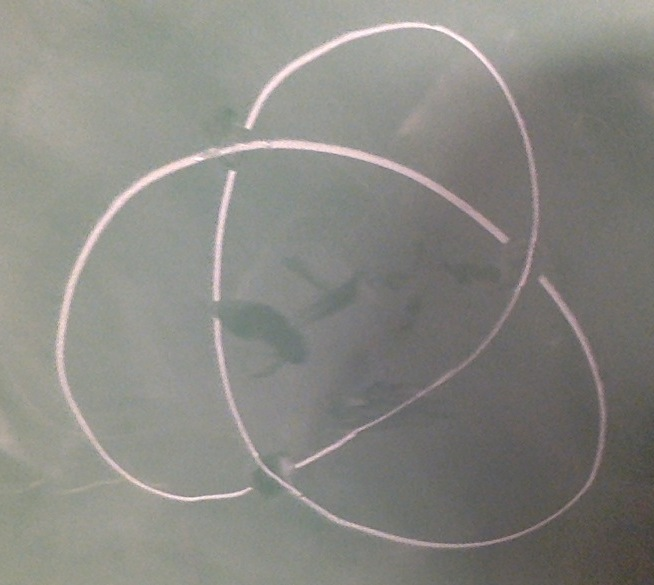
\includegraphics[scale=0.15]{images/trefoil.jpg}

  What is $\fund(\R^3\minus K)$?  Draw two sets of open intervals,
  $A'$ in red and $B'$ in blue, as shown.

  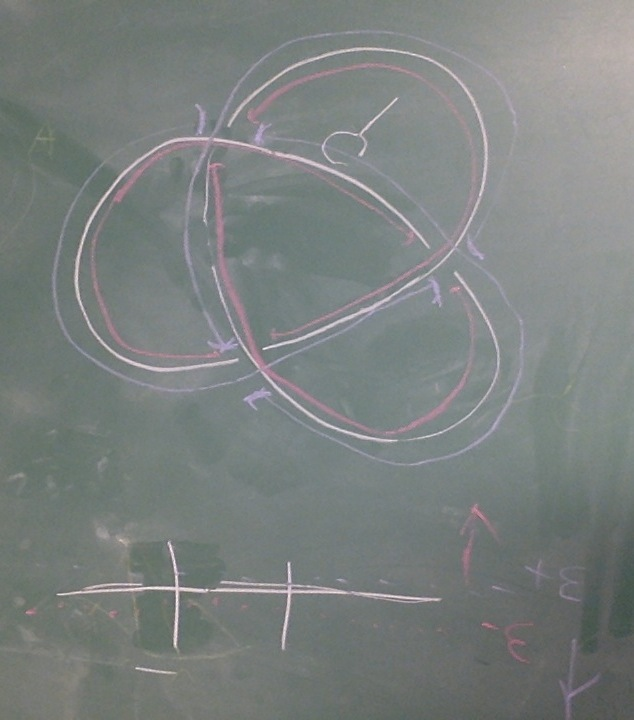
\includegraphics[scale=0.2]{images/trefoil-with-red-and-blue.jpg}

  What looks like the ``ends'' of the ``line segments'' in $A'$, for
  example, are in fact the height of the lines going down to negative
  infinity or up to infinity.  Or you can think of them as ``open
  intervals'', the point being that if there is a little loop (shown
  in white) around one of these, you cannot pull it off the interval,
  since the interval goes on ``forever''.

  $A'$ = $K \cap \{(x,y,z) \in \R^3 \mid z > -\epsilon\}$ ($K$ minus
  the tunnels).

  $B'$ = $K \cap \{(x,y,z) \in \R^3 \mid z < \epsilon\}$ ($K$ minus
  the bridges).

  $A'$ is $m$ open line segments.  In our example, using $K =$
  trefoil, $m = 3$.

  Let $A = (A')^C$.  Then $\fund(A) \isom F_m$, the free group on a
  set of size $m$.

  Let $B = (B')^C$.  Then $\fund(B) \isom F_m$.

  So $A \cap B = \R^3 \minus (A' \union B')$.
  $\fund(A \cap B) \isom F_{2m}$

  ((do we invoke Van Kampen's theorem here?))

  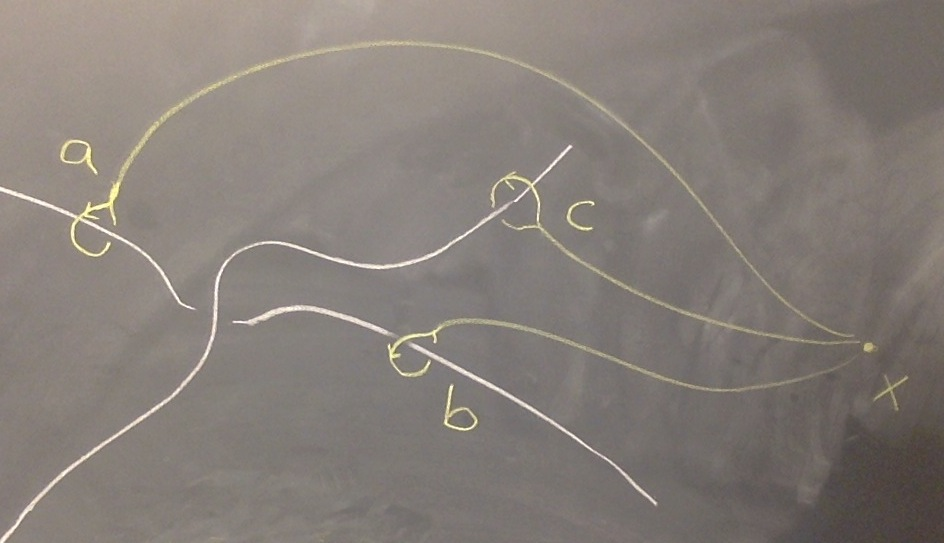
\includegraphics[scale=0.2]{images/mountains.jpg}

  By sliding $a$ under the bridge, we see that $a$ and $b$ are
  conjugate via $c$!

  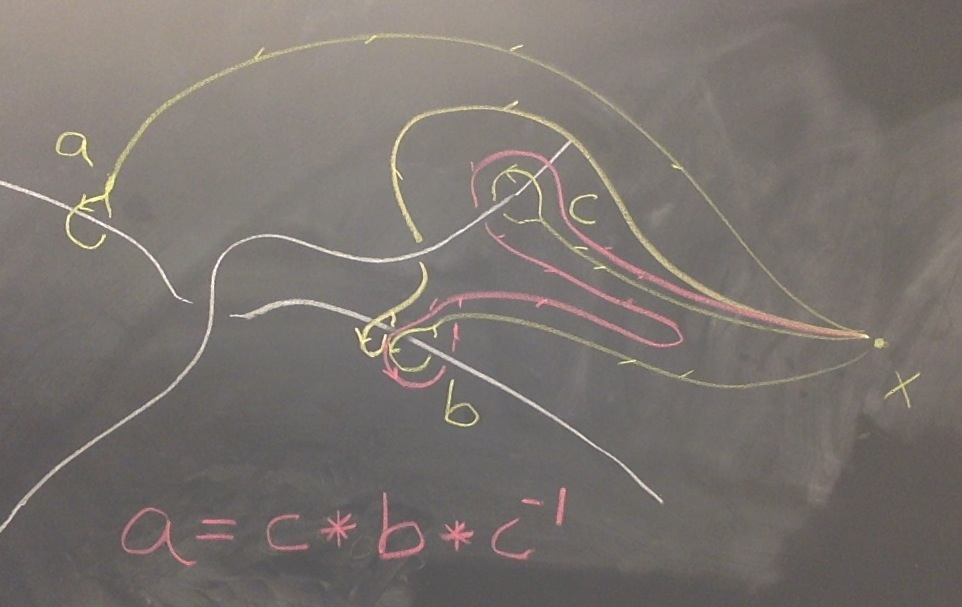
\includegraphics[scale=0.2]{images/mountains-with-explanation.jpg}

  Finally, to compute the fundamental group of $K^C$, we pick an
  arbitrary basepoint $x$ and put loops around the knot as follows.

  We take exactly one loop per open line interval in $A'$.  For each
  crossing, we examine the three loops involved (which are called $a$,
  $b$, and $c$ above) and determine the appropriate conjugate
  relation.  The fundamental group is the group generated by the loops
  and modded out by the relations.

  In the case of the trefoil, the fundamental group
  is $${F_m}/{(a=c*b*c^{-1}, b=a*c*a^{-1}, c=b*a*b^{-1})}$$, as
  illustrated below.

  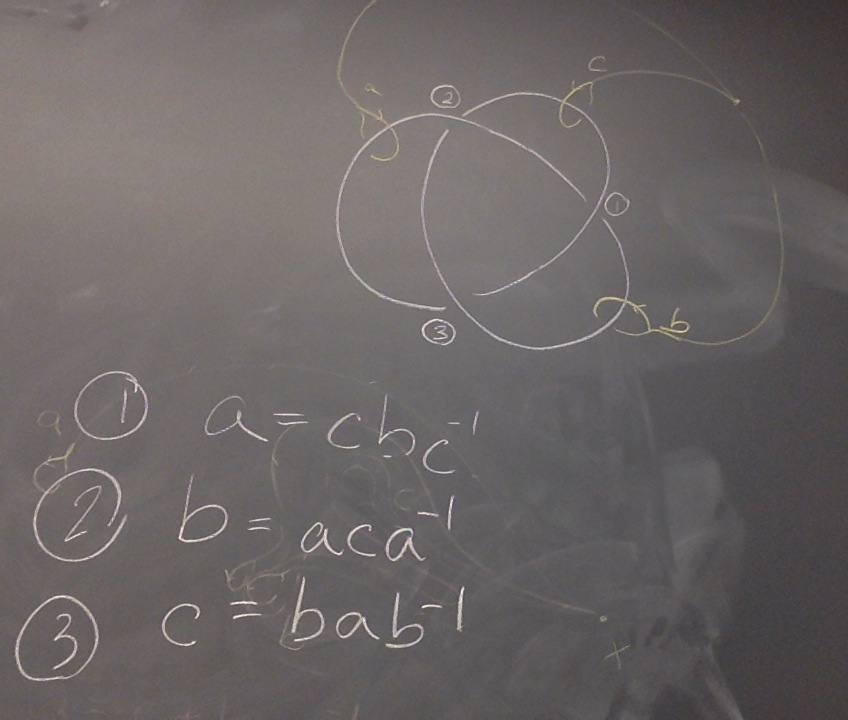
\includegraphics[scale=0.2]{images/trefoil-fully-described.jpg}
\end{example}
\begin{thm}[Wirtinger]
  For any knot $K$, $\fund(\R^3\minus K)$ is generated by loops
  $\gamma_1,,,\gamma_m$ over crossings modulo $a = cbc^{-1}$.
\end{thm}


\section{CW complexes}

CW complexes are like a space built by gluing together balls.
\begin{defn}
  A \de{CW complex} is a space $X$ which is a union of
  $X_0 \subset X_1 \subset \subset \subset$ such that $X_n$ is
  constructed from $X_{n-1}$ by taking
  $X_{n-1} \dunion_{\alpha} D_{\alpha}^n$ modulo identifying $\phi_\alpha \colon S_\alpha^{n-1} \to X_{n-1}$ with $\d D_\alpha^n$.  Note that we are not attaching a $D^n$ to every possible image of $S^{n-1}$, but rather we get to choose which ones we want.

  $X_n$ is called the \de{$n$-skeleton}.  $X$ has topology s.t. $A$ is open iff $A \cap X_n$ is open for all $n$.
\end{defn}
\begin{example}
  $S^n = D^{n-1}/\text{boundary}$ all goes to one point.  $X_0 =$
  discrete set of points.  The $0$-skeleton is a point.  $X_1 =$
  graph. (by connecting the points in $X_0$.)  $X_2 =$ take each cycle
  (can go around multiple times) in $X_1$ and glue it to the boundary
  of a disk (can go around multiple times).
\end{example}
\begin{example}
  ((this example is incomplete and will be repeated next lecture))
  $\R P^n =$ lines in $\R^{n+1}$.

  $\R P^n = \{ \R \dot (1, a_1,,, a_{n-1})\} \isom \R^{n}$.
  $\Union \{ \R \dot (0, a_1,,, a_{n-1})\} \isom \R P^{n-1}$.
\end{example}

\mydate{d7}{6}{2}{2017}

We wish to show how \(\R P^n\) is a \(CW\)-complex. First let the
\(n-1\)-skeleton be \(\R P^{n-1}\). We add the \(n\)-cell \(D^n\) to the
structure under the gluing map \(S^{n} \to \R P^{n-1}\) where
antipodal points are identified. By induction this gives us a
\(CW\)-complex structure.

\begin{example}[Something that does not admit a \(CW\) structure]
  The topological space known as the \emph{Hawaiian earring} is
  constructed as follows.  For each \(n \in \N^{> 0}\) consider the circle of
  radius \(1/n\) tangent to the \(y\)-axis inside the space \(R^2\). All of these circles
  together with the subspace topology yield a topological space \(X\).

  The only hope for putting a \(CW\)-structure on this space would be
  to consider one \(0\)-cell along with a countable amount of
  \(1\)-cells. However, recall that \(CW\)-structures gain their
  topology through the quotient topology, that is, \(\mathcal{O}\) is
  open in \(X\) if and only if \(q^{-1}(\mathcal{O})\) is open, where \(q\) is
  the glueing map. However any open set centered at the origin
  contains an infinite amount of balls, and thus no such
  \(CW\)-structure may be imposed.
\end{example}

Next we show how to compute \(\pi_1\) of a few
\(CW\)-structures. Using Morse Theory one may show that any compact
manifold admits a \(CW\)-structure.

To compute \(\pi_1\) of the torus one can first decompose it as a
\(CW\)-complex as follows
\begin{align*}
  X_0 &= *\\
  X_1 &= S^1 \vee S^1\\
  X_2 &= D_2
\end{align*}

Then we have that \(\pi_1(T^2) = \pi_1(X_1)/\pi_1(A \cap B)\) where
\(B\) is the thickening of the boundary of the square (the square with edges identified to represent the torus) and \(A\) is the thickening of a smaller square
inside of it. \(A\) is clearly contractible.

When talking about moding out by the fundamental group we are really
talking about moding out by the normal subgroup it generates. In
particular this means that conjugation is trivial, and thus we are
free to pick any basepoint we want. This results in
\[\pi_1(T^2) = \left\langle x,y \mid y^{-1}x^{-1}y x = 1 \right\rangle = \Z
    \times \Z\]

\begin{defn}
  The \emph{connected sum} of two topological spaces \(X\) and \(Y\)
  denoted \(X \# Y \) is given by cutting out some neighborhood of
  each \(X\) and \(Y\) and identifying the new boundary.
\end{defn}

It is easy to see that \(T^2 \# T^2\) is the two holed torus, and in general \(\#^n T^2\) is the \(n\) holed torus.

\mydate{e7}{8}{2}{2017}

\section{CW complexes and the fundamental group}

Consider the polygon
\begin{figure}
  % \includegraphics{}
  \label{fig:star}
\end{figure}

$X_0$ = some points

$X_1$ = some paths attached onto those points


\begin{thm}
  If $X$ is a CW complex and $A$ a contractible subcomplex, $\fund(X) = \fund(X/A)$.
\end{thm}
\begin{rmk}
  If $X$ is a CW complex and $A$ a contractible subcomplex, then $X$ is \textbf{not} equal to $X/A$, but $X$ \textbf{is} homotopy equivalent to $X/A$. (this is the quotient by the equivalence relation $x \sim x'$ iff $x = x'$ or $x, x' \in A$).
\end{rmk}

Once we hit $X_1$, the connected components of the complex are determined.

That's because for any $n$-dimensional disk where $n \geq 2$, it's boundary is connected, so that boundary must lie entirely in \textbf{one} of the connected components.

In $\ref{fig:star}$, the set of connected components is $\fund[0](X_0) = \fund[0](X_1)$ ((let's make the fund command take in an optional argument, which will be the subscript of the pi))

If $X_0 = \{[*]\}$ (a single point), then $\fund(X_1) \isom F_{\text{set of 1-cells}}$

$\fund\left( \frac{X_1 \union D^2}{\sim} \right) \isom \frac{\fund(B) * \fund(A)}{A \cap B} \isom \frac{\fund(X_1)}{[\phi] = 1}$, where * denotes the free group product.

In general, I have many gluing maps $\phi_\alpha\from S^1 \to X_1$ and I glue $D^2\alpha$ along $\phi_\alpha(S^1)$.  So $\fund(X_2) \isom \fund(X_1)/\langle[\phi_\alpha]\rangle$.  So when you ``glue'' in a $D^2$, since each $D^2$ is contractible, a path along the boundary of the $D^2$ is now the identity. In other words, each $D^2$ adds a relation!  This is formalized in the following...

\begin{thm}[Not to be proven]
  Every group is the fundamental group of some CW complex.  Construct as follows:

  $X_0$ = point

  $X_1$ = every element in the group gets a loop (the free group)

  $X_2$ = every entry in the multiplication table gets a disk (a relation)

  So it's just like a group presentation!
\end{thm}
\begin{thm}
  Every finitely presented group is the fundamental group of a finite CW complex.
\end{thm}
\begin{thm}
  If $n > 3$, then for any finitely presented group $G$, there exists
  a compact manifold $M$ such that $G \isom \fund(M)$.
\end{thm}
\begin{proof}
  If $n > 2$ and $M$ and $N$ are $n$-manifolds, then consider $M \#
  N$. Recall that $\fund(M \# N) \isom \fund(M) * \fund(N)$. In
  particular, we note that $\fund(\#^n (S^{n-1} \times S^1)) \isom
  F_n$.

  % \includegraphics{} ((that puncture-glueing thing))

  Finally, note that $\d(S^0 \x D^n) = S^0 \x S^{n-1} \setminus
  \d(D^1 \x S^{n-1})$ (If you really want, you can break these
  previous facts into lemmas.)

  % Here is where the actual proof starts.
  Let $M = \#^r (S^1 \times S^{n-1})$ be an $n$-manifold and $n > 3$
  with $r$ the number of generators in the presentation of our group.
  Now, consider a non-self-intersecting loop

  $\alpha \subset U \isom S^1 \x D^{n-1}$ where $U$ comes from the
  tubular neighborhood theorem applied to $\alpha$.

  Then, we get that $\d(D^2 \x S^{n-2}) \isom \d U \isom S^1 \x
  S^{n-2}$.

  % For $n = 2$

  % <picture of cylindar> ((yeah so basically it's this proof that doesn't make sense to me at all.))

  Thus, $\widetilde{M} = \frac{{(M \setminus U) \dunion (D^2 \x S^{n-2})}}{\sim} = \left( M
    \setminus U \right) \union \left( D^2 \times S^{n-2}
  \right)$. Now, to complete the proof, we wish to compute
  $\fund(\tilde{M})$ using Van Kampen's theorem. So, this tells us
  that \[
    \fund(\widetilde{M}) \isom \frac{\fund(M \setminus U) * \fund(D^2
      \times S^{n-2})}{\fund((M \setminus U) \cap (D^2 \times S^{n-2}))}.
  \]
  So, we note that $(M \setminus U) \cap (D^2 \times S^{n-2})$ is
  homotopically equivalent to $S^1 \times S^{n-2}$ and that $(M
  \setminus U) \# (D^2 \times S^{n-2})$ is homeomorphic to
  $M$. Thus, \[
\fund(\widetilde{M}) \isom \frac{\fund(M \setminus U) * \fund(D^2
      \times S^{n-2})}{\fund((M \setminus U) \cap (D^2 \times
      S^{n-2}))} \isom \frac{\fund((M \setminus U) \# (D^2 \times
      S^{n-2}))}{\fund(S^1 \times S^{n-2})} \isom \frac{\fund(M)}{\langle [\alpha] \rangle}
  \]
  and thus, $\fund(\widetilde{M})$ is isomorphic to the free group on
  our generators with one relation given by $[\alpha]$. We can repeate
  this process repeatedly until we get all our relations.
\end{proof}
\begin{thm}
  $\fund(X^2) \isom \fund(X)$ ((this is weird.  is $X^2$ derived from $X$ ?  Like does $X$ denote the entire CW complex, and $X^2$ just a piece of it or something?))
\end{thm}
\begin{proof}
  $\fund(X_{n-1}) \isom \fund(X_n)$.  $n \geq 3$.
  Why does gluing on a higher level dimension disk not affect $\fund$?  It's because the boundary is simply connected.

  $A$ = small disk in A homotopic *
  $B$ = complement of a small disk homotopic $X^{n-1}$ ((i mean i think he meant underscore...))

  $S^{n-1} \to x^{n-1}$.

  $A \cap B \homotopic S^{n-1}$
\end{proof}
\begin{rmk}
  Once $n$ reaches $4$, all bets are off ;(
\end{rmk}



\mydate{d10}{17}{2}{2017}

\begin{thm}
  (Continued from last time) Given $X$ is connected and SLSC, and $p1$ and $p2$ are covering maps, then if a map from $X_1$ to $X_2$ exists, it must be unique and is $\fund$ - equivariant.
\end{thm}

% \includegraphics{} % picture of paths in X, X1, X2.  including alpha, etc.

(AGAIN FROM LAST TIME)
\begin{thm}
  The category of covers of $X$ is equivalent to the category of $\fund$-sets.
\end{thm}

Recall given $H \subset \fund(X, x_0)$, then
$$X_H := X_{\fund/H} = \frac{X^U \x \fund/H}{\fund} = X^U/H$$

\begin{align}
  &\quad (q, \alpha H) \\
  &=(q\alpha, H) \\
  &=(q\alpha h, H)
\end{align} for all $h \in H$.

Note.  If $G/H \isom G/H'$ where $H \mapsto gH'$, then $\Stab(H) = H$, $\Stab(gH') = gH'g^{-1}$, and $H = gH'g^{-1}$.

\begin{thm}
  $X^U/H \isom X^U/H'$ as covers iff $H$ and $H'$ are conjugate.  In which case, $\fund[1](X^U/H) \isom H$.
\end{thm}
\begin{proof}
  There is a natural map $$\fund[1](X^U/H, (q_0, H)) \to \fund(X_1, x_0)$$ where the image of the domain is $H$!

  $p_h^{-1}(x_0) = \{ (q_0, gH) \}_{gH \in G/H}$

  $gHg^{-1} \isom \fund(X^U/H, (q_0, gH) ) \to \fund(X_1, x_0)$

  % \includegraphics{} % fractal picture labelled "X^U" and "\fund \isom F_2"
\end{proof}
\begin{example}
  We will use $H =  \langle a \rangle $ in our image above.

  Note that $ \langle a \rangle $ is just a loop.

  Now look at the image of $\fund(X^U/ \langle a \rangle )$.

  % \includegraphics{} % loop thing w/ two trees

  Note that this is homotopic to a loop!  Woohoo!
\end{example}
\begin{example}
  % \includegraphics{} % loopy pic

  $1 \mapsto a$

  $2 \mapsto b^2$

  $3 \mapsto b^{-1} a b$

  index two normal subgroup

  $F_2 \to \Z/2\Z$

  $a \mapsto 0$

  $b \mapsto 1$
\end{example}


$\#p^{-1}(x) = \#$ of sheets in cover.  $X_S$ is a $\#S$-sheeted cover.  $X_H$ is a $[G:H]$ sheeted cover.

Note: very similar to Galois theory.

topological spaces $\bij$ fields

covers $\bij$ field extensions

$\fund(X)$ $\bij$ absolute Galois group

deck transformations of $X$ $\bij$ field extension automorphism

universal cover $\bij$ algebraic closure

theorem about covers and subgroups $\bij$ fundamental theorem of Galois theory



\mydate{d11}{20}{2}{2017}

\mydate{d12}{22}{2}{2017}

\begin{defn}
  Given a metric space, \de{positive curvature} is when straight lines (going through the same point $p$) don't depart from eachother linearly like in 0 curvature, but get closer to each other than that.  Curvature is a \textbf{local} property, so we only care about what happens as you are first leaving $p$.
\end{defn}

Distance between two points on a graph is merely the length of the shortest path between the two points on the graph.  Again, since curvature is a local property, this means that graphs have a very negative curvature!

\begin{thm}
  The fundamental group of a graph is obtained by ``pruning'' the graph of all branches.  What is left is cycles and paths between those cycles.  The paths between may be contracted to a point.  The result is a jumble of cycles, which can be organized via contraction and homotopy into a single vertex with loops.

  The funamental group will always be $F_n$ for some $n$.
\end{thm}
\begin{thm}
  A topological space $X$ is a graph iff $X^u$ is a tree.
\end{thm}
\begin{defn}
  Given a graph $(V, E)$, an \de{automorphism} is a bijection $f \from V \bij V$ and the induced $E \to E$ such that $a \adj b \in V$ iff $f(a) \adj f(b)$.  (note that $\adj$ denotes adjacency)
\end{defn}
\begin{rmk}
  In other words, $f(\Gamma) = \Gamma$, up to graph isomorphism.  See~\cite{GA} for elaboration.
\end{rmk}
\begin{defn}
  \de{A group $G$ acts on a graph $\Gamma$} if there is a homomorphism $h \from G \to \Aut(\Gamma)$.
\end{defn}
\begin{rmk}
  That is, each element $g$ performs an automorphism on $\Gamma$.  For any vertex $v$ or edge $e$, we can write $g(v)$ or $g(e)$ to denote where $g$ sends $v$ or $e$, respectively.
\end{rmk}

If $G$ is a group acting freely on a graph $\Gamma$, then by definition, $g(v) \cap v = \null$.  If we include the ``edge ends'' touching $v$ in the above, the intersection is still empty.

Now $\Gamma/G$ is the set of orbits.  But there is a different way to interpret $\Gamma/G$.  Take the original $\Gamma$, and for each orbit, collapse all the vertices in that orbit into a single vertex (with induced movement on the edges ((do edges collapse too?))).  The result is again a graph, and so $\Gamma \to \Gamma/G$ is a covering map.

If additionally $\Gamma$ is a tree, then $\Gamma \to \Gamma/G$ is a universal covering map.

\begin{thm}
  ((this theorem doesn't make sense.  if Gamma is a tree, and G acts freely, what automorphisms exist on a tree with no fixed points?.  Even if you find one, it seems that $\fund(\Gamma/G)$ would be trivial, which is a contradiction.))
  If $G$ acts freely on a tree $\Gamma$, then $G$ is free.  Specifically, $$G \isom \fund(\Gamma/G) \isom F_n$$.
\end{thm}
\begin{rmk}
  Note.  If $\Gamma$ is not a tree, then $G$ could be anything.
\end{rmk}

$1 \to K \to F_n \to G \to 1$

If $\Gamma$ is a tree that $F_n$ acts on, then $G$ acts on $\Gamma/K$.

\begin{defn}
  The \de{$n$-flower} is a graph with $1$ vertex and $n$ edges.  (Note that all edges are loops.)
\end{defn}
\begin{thm}[Nielson Schreier]
  ((This theorem doesn't make sense either))
  Subgroups of free groups are free.  Furthermore, a subgroup of finite index has rank determined by the index.  That is, in $F_n$, a subgroup of index $k$ has rank $k(n-1)+1$.
\end{thm}
\begin{proof}
  $\fund(n\text{-flower}) \isom F_n \supset H \isom \fund(k\text{-sheeted cover}) \isom \fund(\text{$k$ vertices, $nk$ edges}) \isom \fund(\text{$nk - k + 1$-flower}) \isom F_{nk - k + 1}$

  Picture this.  A connected graph with $k$ vertices and $nk$ edges.  Now take a path (with $k-1$ edges) that connects all $k$ vertices.  Contract the path to a single vertex.  Now there are only $nk - (k-1)$ edges left, and they are all loops!

((what remains unclear is $F_n \supset H$.  Should it be facing the other way?  It is crucial to understand this argument.))
\end{proof}

\begin{defn}
  A space $X$ is \de{$K(G,1)$} if $\fund(X) \isom G$ and the universal cover of $X$ is contractible.
\end{defn}
Note.  The space is unique up to homotopy equivalence.
\begin{example}
  \begin{itemize}
    \item
    $K(F_n, 1) \isom n$-flower.

    \item
    $K(\Z, 1) \isom S^1$

    \item
    $K(\Z^n, 1) \isom (S^1)^n$

    \item
    $K(G, 1) \isom$ a $g$-holed torus (or non-orientable surface $\not\isom \R P^1$)

    $G = \langle a_1,b_1,,,a_g,b_g \st [a_1,b_1]\ldots[a_g,b_g] = e \rangle$
  \end{itemize}
\end{example}

Given $G$, think of each element as a generator.

So if $g_1, g_2 \in G$, then $g_1$, $g_2$, and $g_1g_2$ are all generators!  They each get a loop!.  But then, of course, we will need to glue faces to build the group.

% \includegraphics[options]{name} pretty picture

So for example, $g_1.g_2 = g_1g_2$, where the LHS is the directed edge concatenation, and the RHS is its very own directed edge.  The picture for this is the triangle.

Similarly, we can create higher dimensional simplices.  For example
$g_1g_2g3 = g_1.(g_2g3)$
in the tetrahedron simplex (see pic).

I have an $n$-cell for every $n$-tuple

$D^n \isom \{ (x_0,,,x_n) \in \R^{n+1} \st \sum x_i = 1, x_i \geq 0 \}$

If one of the coordinates is 0, we get a lower $d$-simplex.





\mydate{d13}{24}{2}{2017}

\section*{Simplicial homology}

The fundamental group associates to a topological space (a not
necessarily abelian) group, however we have already seen that this
comes with many insufficiency. For example, the fundamental group
fails to detect the cell structure beyond \(2\)-cells. One way to get
around this problem is to consider the higher homotopy groups, defined
in an analogous way. While these groups are able to detected the
higher dimensional cell structure, they are very difficult to compute.

We will now begin to develop the theory of homology, which is much
easier to compute with. However this easy of use comes with a cost, in
particular, the basic definitions are more complicated. Instead of
attaching to a given topology space a single group, we will attach a
chain of abelian subgroups.

Define the \(n\)-simplex to be the smallest convex figure in
\(\R^{n+1}\) that does not lay completely in any \(n\)-dim
hyper-plane. In practice just think \(0\)-simplex is a point
\(1\)-simplex is a line, \(2\)-simplex is a triangle, \(3\)-simplex is
a pyramid, etc. Now what Hatcher calls a face is more generally
commonly referred to as a facet. Normally a face refers to any part of
the boundary of the simplex, while facet specifically refers to the
faces of dimension \(n-1\). Another way to say this is that a facet is
a maximal face. In general usage face includes all of the following
\(\emptyset\), vertices, edges, and yes even facets.

We will start with simplicial homology as it appears to be more tame
(key word being appears), than singular homology. However singular
homology is defined in such a way that many important properties are
immediately apparent (i.e. homotopy invariance).

Built out of \(n\)-simplices are simplicial-complexes, however we will
study Hatcher's \(\Delta\)-complex which is more convenient to work with. 

\mydate{d14}{27}{2}{2017}

\begin{rmk}
  Hatcher created the notion of Delta-complexes because they are more
  convenient than simplicial complexes.  The following are examples of
  $\Delta$-complexes that are not simplicial complexes.
  \begin{itemize}
  \item 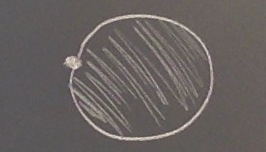
\includegraphics[scale=0.22]{images/not-delta-complex1}
  \item 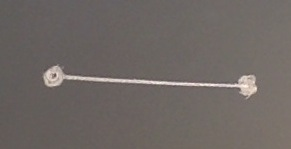
\includegraphics[scale=0.2]{images/not-delta-complex2}
  \item 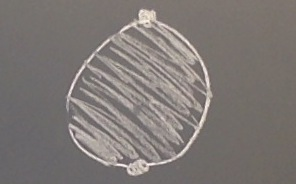
\includegraphics[scale=0.2]{images/not-delta-complex3}
  \end{itemize}
  $\Delta$-complexes allow you to glue vertices together, but
  simplicial complexes do not. ((John Harnois))
\end{rmk}

An $n$-chain (non-rigorous idea) is a union (with multiplicity, and
negative multiplicity) of $n$-simplices.  Therefore, an $n$-chain is a
subspace of dimension $n$.  Also, negative multiplicities represent
the opposite orientation of their positive counterparts.

An orientation of an $n$-simplex is specified by an order on the
vertices.  Also, an even permutation (on these vertices) is
orientation preserving, while an odd permutation is orientation
reversing.  By convention in Hatcher (and this course), faces are
oriented according to the induced order from their vertices.

\begin{defn}
  \de{The group of $n$-chains} \de{$\Delta_n(X)$} is the free abelian
  group with basis the open $n$-simplices $e_\alpha^n$ of $X$.  An
  element of $\Delta_n(X)$ is an \de{$n$-chain}, and is written
  $\sum_\alpha n_\alpha e_\alpha^n$ with coefficients
  $n_\alpha \in \Z$.
\end{defn}
\begin{rmk}
  Equivalently, we could write $\sum_\alpha n_\alpha \sigma_\alpha$
  where $\sigma_\alpha \from \Delta^n \to X$ is the characteristic
  map.

  If there do not exist any $n$-dim simplices, then
  $\Delta_n(X) = \{0\}$.
\end{rmk}

\begin{defn}[boundary of an oriented $n$-simplex]
  The boundary of an $n$-simplex $[0, 1,,, n]$ is defined by
  $$\d([0, 1,,, n]) := \sum_{i=0}^n (-1)^i [0, 1,,, \hat{i},,, n]$$
\end{defn}
\begin{defn}[boundary of an $n$-chain]
  The boundary map $\d \from \Delta_n(X) \to \Delta_{n-1}(X)$ is
  linear, and so
  $$\d(\sum_\alpha n_\alpha e_\alpha^n) := \sum_\alpha n_\alpha
  \d(e_\alpha^n)$$
\end{defn}

Houston we have a problem.  The induced orientation on the boundary
doesn't neccessarily agree with the original orientation on the those
lower dimensional simplices!  (See above).  So what to do?  I think
that's where the $(-1)^i$ comes into play.

\begin{example}[Hatcher, p.105]
  \quad

  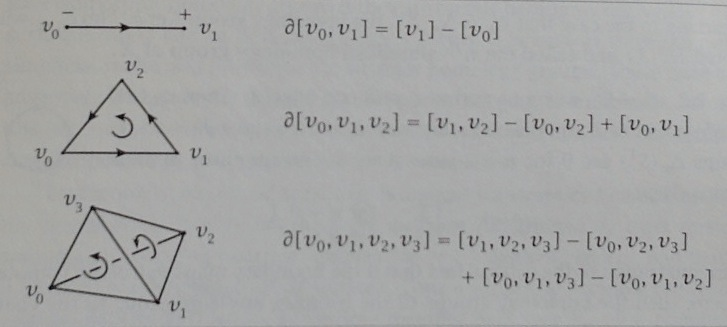
\includegraphics[scale=0.5]{images/boundary-of-oriented-simplex}
\end{example}

\begin{example}
  % pretty picture
  $$\d(X) = - a - b + c$$
  $$\d(Y) =$$

  $\sigma$ is the glueing map!  not a permutation!
  $\sigma \from \Delta^n \to X$.  where $[0, 1, 2]$ denotes the
  simplex.
\end{example}

Claim: $\d^2 = 0$.

\begin{defn}
  $$H_n^\Delta(X) := \ker(\d \from \Delta_n \to \Delta_{n-1})/\im(\d \from \Delta_{n+1} \to \Delta_{n})$$
\end{defn}

\begin{example}
  $H_2^\Delta(K^2) = 0$ $H_1^\Delta(K^2) \isom \Z \oplus \Z/2\Z$
  $H_0^\Delta(K^2) = \Z$

  where $\Z^2 \to(overset [-1 -1; -1 1; 1 1]) \Z^3 \to(overset 0) \Z$

  $[0 2 0]^transpose$
\end{example}




\mydate{d15}{1}{3}{2017}

\mydate{d16}{3}{3}{2017}

When using normal subgroups that corr to covering spaces, you get
maximal symmetry. It looks the same at every point. It's the same as
taking universal cover and modding out by relations.

When you use regular subgroups that correspond to covering spaces, you cannot
do the modding out trick.  (or maybe you can only do it locally).  It
won't be symmetric.  It will look like example (a) in Hatcher for $S^1 \vee
S^1$.


\section*{Singular homology}

\begin{defn}
  A \de{singular $n$-chain} has the same definition as an $n$-chain, except that the maps from $\Delta^n \to X$ have no restrictions other than continuity.
\end{defn}
\begin{rmk}
  Unlike a $\Delta$-complex, no injectivity is required on the interior!
  \begin{itemize}
    \item There are uncountably many complexes for all interesting spaces!
    \item There are simplices of all dimensions in $\N$.
  \end{itemize}
\end{rmk}


The definition of $homology$ $H_n(X) = \frac{}{}$ is the same as before, but now notice that these $H$'s can be really big!

If $X$, $Y$ are spaces and $f \from X \to Y$, then I have an induced map $$C_n(X) \to C_n(Y)$$ where $$ \sigma \mapsto f \of \sigma$$ obviously commutes with $\d$.

\begin{thm}
  $f$ induces a map $$f_\alpha \from H_n(X) \to H_n(Y)$$ and $$(f \of g)_\ast = f_\ast \of g_\ast$$
\end{thm}


\mydate{d17}{13}{3}{2017}

\mydate{d18}{15}{3}{2017}

\mydate{d19}{17}{3}{2017}

\mydate{d20}{20}{3}{2017}

\mydate{d21}{22}{3}{2017}

\mydate{d22}{24}{3}{2017}

\mydate{d23}{27}{3}{2017}

\mydate{d24}{29}{3}{2017}

\mydate{d25}{31}{3}{2017}




\begin{bibdiv}
\begin{biblist}
% THIS SHOULD BE MOVED TO A SEPARATE FILE IF IT GETS TOO CUMBERSOME
% see http://ctan.math.utah.edu/ctan/tex-archive/macros/latex/contrib/amsrefs/amsrdoc.pdf
  \bib{ncatlab}{webpage}{
    title={Joyal's CatLab},
    url={https://ncatlab.org/joyalscatlab/published/Categories},
    accessdate={2017-02-06},
    date={2010-05-30},
  },
  \bib{functors}{webpage}{
    title={Joyal's CatLab},
    url={https://ncatlab.org/joyalscatlab/published/Functors},
  },
  \bib{GA}{webpage}{
    title={Graph Automorphism},
    url={http://mathworld.wolfram.com/GraphAutomorphism.html},
    accessdate={2017-02-22},
    author={Weisstein, Eric W.},
  },
  \bib{Hatcher}{book}{
    title={Algebraic Topology},
    author={Hatcher, Allen},
    publisher={Cambridge University Press},
    date={2002},
  },
\end{biblist}
\end{bibdiv}


\end{document}

%%% Local Variables:
%%% mode: latex
%%% TeX-master: "algebraic-topology.tex"
%%% End:
